\documentclass[10pt]{article}
\usepackage{amsmath}
\usepackage{amsthm}
\usepackage{amsfonts}
\usepackage{amssymb}
\usepackage{amssymb}
\usepackage{booktabs}
\setlength\parindent{0pt}
\usepackage[margin=1.2in]{geometry}
\usepackage{enumitem}
\usepackage{mathtools}
\mathtoolsset{showonlyrefs=true}
\usepackage{pdflscape}
\usepackage{xcolor}
\usepackage{hyperref}
\setcounter{tocdepth}{4}
\setcounter{secnumdepth}{4}
\usepackage[listings,skins,breakable]{tcolorbox} % package for colored boxes
\usepackage{etoolbox}
\usepackage{placeins}
\usepackage{tikz}
\usepackage{color}  % Allows for color customization
\usepackage{subcaption}
\usepackage[utf8]{inputenc}


% Make it so that the bottom page of a 
% book section doesn't have weird spacing
\raggedbottom


% Define custom colors
% You can-redo these later, they're not being used 
% for anything as of 5/12/24
\definecolor{codegreen}{rgb}{0,0.6,0}
\definecolor{codegray}{rgb}{0.5,0.5,0.5}
\definecolor{codepurple}{rgb}{0.58,0,0.82}
\definecolor{backcolour}{rgb}{0.95,0.95,0.92}

% You can-redo the lstlisting style later, it's not being used 
% for anything as of 5/12/24

% Define the lstlisting style
\lstdefinestyle{mystyle}{
    backgroundcolor=\color{backcolour},   
    commentstyle=\color{codegreen},
    keywordstyle=\color{magenta},
    numberstyle=\tiny\color{codegray},
    stringstyle=\color{codepurple},
    basicstyle=\ttfamily\footnotesize,
    breakatwhitespace=false,         
    breaklines=true,                 
    captionpos=b,                    
    keepspaces=true,                 
    numbers=left,                    
    numbersep=5pt,                  
    showspaces=false,                
    showstringspaces=false,
    showtabs=false,                  
    tabsize=2
}
\lstset{style=mystyle}


% Set the length of \parskip to add a line between paragraphs
\setlength{\parskip}{1em}


% Set the second level of itemize to use \circ as the bullet point
\setlist[itemize,2]{label={$\circ$}}

% Define symbols
\DeclareMathSymbol{\Perp}{\mathrel}{symbols}{"3F}
\newcommand\barbelow[1]{\stackunder[1.2pt]{$#1$}{\rule{.8ex}{.075ex}}}
\newcommand{\succprec}{\mathrel{\mathpalette\succ@prec{\succ\prec}}}
\newcommand{\precsucc}{\mathrel{\mathpalette\succ@prec{\prec\succ}}}


\newcounter{example}[section] % Reset example counter at each new section
\renewcommand{\theexample}{\thesection.\arabic{example}} % Format the example number as section.number

\newenvironment{example}
  {% Begin environment
   \refstepcounter{example}% Step counter and allow for labeling
   \noindent\textbf{Example \theexample.} % Display the example number
  }
  {% End environment
   \par\noindent\hfill\textit{End of Example.}\par
  }



% deeper section command
% This will let you go one level deeper than whatever section level you're on.
\makeatletter
\newcommand{\deepersection}[1]{%
  \ifnum\value{subparagraph}>0
    % Already at the deepest standard level (\subparagraph), cannot go deeper
    \subparagraph{#1}
  \else
    \ifnum\value{paragraph}>0
      \subparagraph{#1}
    \else
      \ifnum\value{subsubsection}>0
        \paragraph{#1}
      \else
        \ifnum\value{subsection}>0
          \subsubsection{#1}
        \else
          \ifnum\value{section}>0
            \subsection{#1}
          \else
            \section{#1}
          \fi
        \fi
      \fi
    \fi
  \fi
}
\makeatother


% same section command
% This will let create a section at the same level as whatever section level you're on.
\makeatletter
\newcommand{\samesection}[1]{%
  \ifnum\value{subparagraph}>0
    \subparagraph{#1}
  \else
    \ifnum\value{paragraph}>0
      \paragraph{#1}
    \else
      \ifnum\value{subsubsection}>0
        \subsubsection{#1}
      \else
        \ifnum\value{subsection}>0
          \subsection{#1}
        \else
          \ifnum\value{section}>0
            \section{#1}
          \else
            % Default to section if outside any sectioning
            \section{#1}
          \fi
        \fi
      \fi
    \fi
  \fi
}
\makeatother

\makeatletter
\newcommand{\shallowersection}[1]{%
  \ifnum\value{subparagraph}>0
    \paragraph{#1} % From subparagraph to paragraph
  \else
    \ifnum\value{paragraph}>0
      \subsubsection{#1} % From paragraph to subsubsection
    \else
      \ifnum\value{subsubsection}>0
        \subsection{#1} % From subsubsection to subsection
      \else
        \ifnum\value{subsection}>0
          \section{#1} % From subsection to section
        \else
          \ifnum\value{section}>0
            \chapter{#1} % Assuming a document class with chapters
          \else
            \section{#1} % Default to section if somehow higher than section
          \fi
        \fi
      \fi
    \fi
  \fi
}
\makeatother



\newcounter{problemcounter}
\renewcommand{\theproblemcounter}{Q.\arabic{problemcounter}}

% Define the problem environment
\newenvironment{problem}[1][]{%
  \refstepcounter{problemcounter}%
  \if\relax\detokenize{#1}\relax
    \tcolorbox[breakable, colback=red!10, colframe=red!50, fonttitle=\bfseries, title={Problem \theproblemcounter}, arc=5mm, boxrule=0.5mm]
  \else
    \tcolorbox[breakable, colback=red!10, colframe=red!50, fonttitle=\bfseries, title={Problem \theproblemcounter: #1}, arc=5mm, boxrule=0.5mm]
    \addcontentsline{toc}{subsubsection}{\theproblemcounter: #1}%
  \fi
}{
  \endtcolorbox
}

% Define a new counter for definitions
\newcounter{definitioncounter}
\renewcommand{\thedefinitioncounter}{D.\arabic{definitioncounter}}

\newenvironment{definition}[1][]{%
  \refstepcounter{definitioncounter}%
  \if\relax\detokenize{#1}\relax
    \tcolorbox[
      breakable,
      parbox=false, % Treat content normally regarding paragraphs
      before upper={\parindent0pt \parskip7pt}, % No indentation and add space between paragraphs
      colback=blue!10,
      colframe=blue!50,
      fonttitle=\bfseries,
      title={Definition \thedefinitioncounter},
      arc=5mm,
      boxrule=0.5mm,
      before skip=10pt, % Adjust vertical space before the box
      after skip=10pt % Adjust vertical space after the box
    ]
  \else
    \tcolorbox[
      breakable,
      parbox=false,
      before upper={\parindent0pt \parskip7pt},
      colback=blue!10,
      colframe=blue!50,
      fonttitle=\bfseries,
      title={Definition \thedefinitioncounter: #1},
      arc=5mm,
      boxrule=0.5mm,
      before skip=10pt,
      after skip=10pt
    ]
  \fi
}{
  \endtcolorbox
}


% Define a new counter for theorems
\newcounter{theoremcounter}
\renewcommand{\thetheoremcounter}{T.\arabic{theoremcounter}}

\newenvironment{theorem}[1][]{%
  \refstepcounter{theoremcounter}%
  \if\relax\detokenize{#1}\relax
    \tcolorbox[
      breakable,
      parbox=false, % Treat content normally regarding paragraphs
      before upper={\parindent0pt \parskip7pt}, % No indentation and add space between paragraphs
      colback=green!10,
      colframe=green!55,
      fonttitle=\bfseries,
      title={Theorem \thetheoremcounter},
      arc=5mm,
      boxrule=0.5mm,
      before skip=10pt, % Adjust vertical space before the box
      after skip=10pt % Adjust vertical space after the box
    ]
  \else
    \tcolorbox[
      breakable,
      parbox=false,
      before upper={\parindent0pt \parskip7pt},
      colback=green!10,
      colframe=green!55,
      fonttitle=\bfseries,
      title={Theorem \thetheoremcounter: #1},
      arc=5mm,
      boxrule=0.5mm,
      before skip=10pt,
      after skip=10pt
    ]
  \fi
}{
  \endtcolorbox
}


% Define a new counter for remarks
\newcounter{remarkcounter}
\renewcommand{\theremarkcounter}{R.\arabic{remarkcounter}}

\newenvironment{remark}[1][]{%
  \refstepcounter{remarkcounter}%
  \if\relax\detokenize{#1}\relax
    \tcolorbox[
      breakable,
      parbox=false, % Treat content normally regarding paragraphs
      before upper={\parindent0pt \parskip7pt}, % No indentation and add space between paragraphs
      colback=green!10,
      colframe=green!55,
      fonttitle=\bfseries,
      title={Remark \theremarkcounter},
      arc=5mm,
      boxrule=0.5mm,
      before skip=10pt, % Adjust vertical space before the box
      after skip=10pt % Adjust vertical space after the box
    ]
  \else
    \tcolorbox[
      breakable,
      parbox=false,
      before upper={\parindent0pt \parskip7pt},
      colback=green!10,
      colframe=green!55,
      fonttitle=\bfseries,
      title={Remark \theremarkcounter: #1},
      arc=5mm,
      boxrule=0.5mm,
      before skip=10pt,
      after skip=10pt
    ]
  \fi
}{
  \endtcolorbox
}

% Define a new counter for lemmas
\newcounter{lemmacounter}
\renewcommand{\thelemmacounter}{L.\arabic{lemmacounter}}

\newenvironment{lemma}[1][]{%
  \refstepcounter{lemmacounter}%
  \if\relax\detokenize{#1}\relax
    \tcolorbox[
      breakable,
      parbox=false, % Treat content normally regarding paragraphs
      before upper={\parindent0pt \parskip7pt}, % No indentation and add space between paragraphs
      colback=green!10,
      colframe=green!55,
      fonttitle=\bfseries,
      title={Lemma \thelemmacounter},
      arc=5mm,
      boxrule=0.5mm,
      before skip=10pt, % Adjust vertical space before the box
      after skip=10pt % Adjust vertical space after the box
    ]
  \else
    \tcolorbox[
      breakable,
      parbox=false,
      before upper={\parindent0pt \parskip7pt},
      colback=green!10,
      colframe=green!55,
      fonttitle=\bfseries,
      title={Lemma \thelemmacounter: #1},
      arc=5mm,
      boxrule=0.5mm,
      before skip=10pt,
      after skip=10pt
    ]
  \fi
}{
  \endtcolorbox
}

% Define a new counter for propositions
\newcounter{propositioncounter}
\renewcommand{\thepropositioncounter}{P.\arabic{propositioncounter}}

\newenvironment{proposition}[1][]{%
  \refstepcounter{propositioncounter}%
  \if\relax\detokenize{#1}\relax
    \tcolorbox[
      breakable,
      parbox=false, % Treat content normally regarding paragraphs
      before upper={\parindent0pt \parskip7pt}, % No indentation and add space between paragraphs
      colback=green!10,
      colframe=green!55,
      fonttitle=\bfseries,
      title={Proposition \thepropositioncounter},
      arc=5mm,
      boxrule=0.5mm,
      before skip=10pt, % Adjust vertical space before the box
      after skip=10pt % Adjust vertical space after the box
    ]
  \else
    \tcolorbox[
      breakable,
      parbox=false,
      before upper={\parindent0pt \parskip7pt},
      colback=green!10,
      colframe=green!55,
      fonttitle=\bfseries,
      title={Proposition \thepropositioncounter: #1},
      arc=5mm,
      boxrule=0.5mm,
      before skip=10pt,
      after skip=10pt
    ]
  \fi
}{
  \endtcolorbox
}

%\newtheorem{proposition}[theorem]{Proposition}  % Propositions share numbering with theorems


% Define a new counter for notes
\newcounter{notescounter}
\renewcommand{\thenotescounter}{D.\arabic{notescounter}}

\newenvironment{notes}[1][]{
  \refstepcounter{notescounter}%
  \if\relax\detokenize{#1}\relax
    % If #1 is empty, set the title to "Notes"
    \tcolorbox[
      breakable,
      parbox=false, % Treat content normally regarding paragraphs
      before upper={\parindent0pt \parskip7pt}, % No indentation and add space between paragraphs
      colback=blue!10,
      colframe=blue!50,
      fonttitle=\bfseries,
      title={Notes},
      arc=5mm,
      boxrule=0.5mm,
      before skip=10pt, % Adjust vertical space before the box
      after skip=10pt % Adjust vertical space after the box
    ]
  \else
    % If #1 is not empty, use it as the title
    \tcolorbox[
      breakable,
      parbox=false,
      before upper={\parindent0pt \parskip7pt},
      colback=blue!10,
      colframe=blue!50,
      fonttitle=\bfseries,
      title={#1}, % Use provided title instead of default
      arc=5mm,
      boxrule=0.5mm,
      before skip=10pt,
      after skip=10pt
    ]
  \fi
}{
  \endtcolorbox
}







% Define a new counter for questions
\newcounter{questionscounter}
\renewcommand{\thequestionscounter}{D.\arabic{questionscounter}}

\newenvironment{questions}[1][]{
  \refstepcounter{questionscounter}%
  \if\relax\detokenize{#1}\relax
    % If #1 is empty, set the title to "Questions"
    \tcolorbox[
      breakable,
      parbox=false, % Treat content normally regarding paragraphs
      before upper={\parindent0pt \parskip7pt}, % No indentation and add space between paragraphs
      colback=red!10,
      colframe=red!50,
      fonttitle=\bfseries,
      title={Questions},
      arc=5mm,
      boxrule=0.5mm,
      before skip=10pt, % Adjust vertical space before the box
      after skip=10pt % Adjust vertical space after the box
    ]
  \else
    % If #1 is not empty, use it as the title
    \tcolorbox[
      breakable,
      parbox=false,
      before upper={\parindent0pt \parskip7pt},
      colback=red!10,
      colframe=red!50,
      fonttitle=\bfseries,
      title={#1}, % Use provided title instead of default
      arc=5mm,
      boxrule=0.5mm,
      before skip=10pt,
      after skip=10pt
    ]
  \fi
}{
  \endtcolorbox
}






% Define a new counter for overview
\newcounter{overviewcounter}
\renewcommand{\theoverviewcounter}{D.\arabic{overviewcounter}}

\newenvironment{overview}[1][]{%
  \refstepcounter{overviewcounter}%
  \if\relax\detokenize{#1}\relax
    \tcolorbox[
      breakable,
      parbox=false, % Treat content normally regarding paragraphs
      before upper={\parindent0pt \parskip7pt}, % No indentation and add space between paragraphs
      colback=green!10,
      colframe=green!55,
      fonttitle=\bfseries,
      title={Overview},
      arc=5mm,
      boxrule=0.5mm,
      before skip=10pt, % Adjust vertical space before the box
      after skip=10pt % Adjust vertical space after the box
    ]
  \else
    \tcolorbox[
      breakable,
      parbox=false,
      before upper={\parindent0pt \parskip7pt},
      colback=green!10,
      colframe=green!55,
      fonttitle=\bfseries,
      title={Overview},
      arc=5mm,
      boxrule=0.5mm,
      before skip=10pt,
      after skip=10pt
    ]
  \fi
}{
  \endtcolorbox
}



% Add a line after paragraph header
\makeatletter
\renewcommand\paragraph{\@startsection{paragraph}{4}{\z@}%
            {-3.25ex \@plus -1ex \@minus -.2ex}%
            {1.5ex \@plus .2ex}%
            {\normalfont\normalsize\bfseries}}
\makeatother


% Taking away line before and after align
\BeforeBeginEnvironment{align}{\vspace{-\parskip}}
\AfterEndEnvironment{align}{\vskip0pt plus 2pt}

\usepackage{changepage}

\title{Ch. 5 Mediation: Exploring Relevant Mechanisms}

\author{Dylan Baker}

\begin{document}
\maketitle

\section{Introduction}

Mediation analysis 
seeks to answer the question 
``what is the causal pathway from treatment $(D)$ to outcome $(Y)$?''

Running examples:

\begin{itemize}
    \item Scurvy, Lemon Juice, and Vitamin C: 
        Many sailors suffered from scurvy, $Y$. It was identified 
        that lemon juice consumption, $D$, led to a 
        decrease in scurvy. It wasn't until much later that 
        doctors understood that the mediator was vitamin C.
    \item Burland, Dynarski, Michelmore, Owen, Raghuraman (2023)
        conduct a natural field experiment in which they compare 
        college application rates among low-income 
        high school students to the University of Michigan. 
        The two treatments were to either offer free tuition to 
        everyone or to offer free tuition to people who demonstrate 
        need through an application process. They find that both 
        treatments increase application rates, but the
        free tuition for all treatment has a larger effect (28 p.p. over control 
        and 19 p.p. over the need-based treatment). In this case,
        alleviating uncertainty was a partial mediator.
    \item Bursztyn, González, and Yanagizawa-Drott (2020) 
        analyzed the relationship between perceived norms 
        and female labor force participation in Saudi Arabia. 
        They found that most men both thought it was 
        acceptable for women to work outside of the home 
        and underestimated the share of other men who thought the same.
        Implementing the information treatment of clarifying the 
        true share of other men who thought it was acceptable
        increased various outcomes related to the wives of 
        these men working outside of the home. A partial mediator 
        considered here is the change in perceived norms among 
        the \emph{wives} who did not receive the treatment, but 
        may have heard about it from their husbands.
\end{itemize}

\section{Mediation: The Basics of Causal Pathways}

\subsection{Complete or Partial Mediation}

Mediation can be either complete or partial, in which, intuitively, 
the effect of $D$ on $Y$ either flows completely or only partially 
through the mediator $M$.

\begin{itemize}
    \item Lemon Juice and Scurvy: The effect of lemon juice on scurvy is completely mediated 
        by vitamin C. 
    \item Certainty and College Applications: 
        The effect of tuition assistance on 
        college applications is partially mediated by 
        alleviating uncertainty. However, a direct effect of $D$ 
        may also be influential. The book lists: 
        ``the effect of colorful mailings, encouragement to apply, 
        and detailed aid information.'' 
    \item Norms and Female Labor Force Participation: 
        The effect of the information treatment on Saudi Arabian men's 
        willingness to let their wives work via 
        ``relaxing incorrect conformity motives'' 
        is the direct effect.
        A partial mediator is the change in their wives' willingness 
        to work by ``relaxing incorrect conformity motives''
        after hearing about the treatment from their husbands.
\end{itemize}

\begin{questions}
    I'm not sure that I understand at this moment why things 
    like ``colorful mailings'' constitute a direct effect, rather 
    than another mediator.
\end{questions}


\subsection{Decomposing Total Effects in the Presence of Mediators}

As a simple example, suppose there is 
a binary treatment variable, $D$, 
and a binary mediator, $M$.

Define $M_i(d)$ to be the value of the mediator under 
treatment condition $d \in \{0, 1\}$.

Define $Y_i\left(M_i(d), d\right)$ to be the value of the outcome
under treatment condition $d$ and mediator value $M_i(d)$.

There is now no one uncontroversial 
definition of the ATE.

\begin{definition}[Average Direct Effect (ADE)] 
    One ATE iteration that may be of interest in this setting is the
    average direct effect:

    \begin{align}
        \text{ADE}(d) \equiv \mathbb{E}\left[Y_i\left(M_i(d), 1\right)-Y_i\left(M_i(d), 0\right)\right]
    \end{align}

    ``The ADE corresponds to the average effect of treatment once we 
    average over the values of the mediator that arise naturally 
    in the population.''

\end{definition}

\begin{definition}[Average Indirect Effect (AIE)] 
    
    In a similar spirit, we can define the average indirect effect:

    \begin{align}
        \operatorname{AIE}(d) \equiv \mathbb{E}\left[Y_i\left(M_i(1), d\right)-Y_i\left(M_i(0), d\right)\right]
    \end{align}

    which corresponds to the average effect when we hold 
    the treatment condition fixed. 

\end{definition}

In the case of complete mediation, the ADE is zero,
and the AIE holds the total effect.

\begin{example}
    In the Saudi Arabian norms experiment,
   ``$\operatorname{AIE}(0)$ is capturing how much 
    higher (or lower) female labor force participation 
    would be had no husbands received the norms information,
    but had one group had their wives conveyed information 
    as if their husbands had received norms information,
    isolating the potential indirect effect.''
\end{example}

What does our typical ATE capture in this binary mediator scenario?

Notice that you can re-write the ATE as follows:

\begin{align}
        \operatorname{ATE}=&\mathbb{E}\left[Y_i\left(M_i(1), 1\right)-Y_i\left(M_i(0), 0\right)\right] \label{eq:ATE_ex1} \\
        = &\underbrace{\mathbb{E}\left[Y_i\left(M_i(1), 1\right)-Y_i\left(M_i(1), 0\right)\right]}_{\text{ADE}(1)}+\underbrace{\mathbb{E}\left[Y_i\left(M_i(1), 0\right)-Y_i\left(M_i(0), 0\right)\right]}_{\operatorname{AIE}(0)} \label{eq:ATE_ex2} \\
        = &\underbrace{\mathbb{E}\left[Y_i\left(M_i(1), 1\right)-Y_i\left(M_i(0), 1\right)\right]}_{\text{AIE}(1)}+\underbrace{\mathbb{E}\left[Y_i\left(M_i(0), 1\right)-Y_i\left(M_i(0), 0\right)\right]}_{\text{ADE}(0)} \label{eq:ATE_ex3}
\end{align}

Then, the ATE is a sum of the ADE and AIE under different 
treatment conditions.

\subsection{Moving the Goalposts: Controlled and Principal-Strata Effects}

Suppose that we can control both the treatment 
and mediator conditions. Then, we can manipulate each 
in what functionally amounts a 
``full-factorial design in the space of $D \times M$.''

\begin{definition}[Average Controlled Direct Effect (ACDE)] 
    What we may have previously called an interaction effect, 
    we now ``re-interpret'' to as the average controlled direct effect:

    \begin{align}
        \text{ACDE}(m) \equiv \mathbb{E}\left[Y_i(m, 1)-Y_i(m, 0)\right]
    \end{align}

\end{definition}

In practice, this may be hard to attain. 
For one thing, it may be the case that varying the mediator 
is simply not possible for ethical, legal, or practical reasons.
Moreover, if treatments and mediators endogenously interact, 
then the level of the mediator imposed by the researcher may differ
from the level that would have arisen naturally. 
In that case, it may be that $\text{ACDE}(1) \neq \text{ADE}(1)$.
That is, the ``controlled'' effect may differ from the ``organic'' effect,
because the mediator may take on a different level when controlled 
compared to when it organically emerged as a result of the treatment.
This places a responsibility on the researcher to think carefully 
and choose practically interesting levels of the mediator.

\subsubsection{``Always''-Mediator-Takers}

For the subset of the population that always takes the mediator,
i.e., $M(1)=M(0)=1$, the sub-population ATE is the same as the 
sub-population ADE, so we can get:

\begin{align}
    \text { subpopulation ATE} & =\mathbb{E}\left[Y_i\left(M_i(1), 1\right)-Y_i\left(M_i(0), 0\right) \mid M_i(1)=M_i(0)=1\right] && \text{From } \eqref{eq:ATE_ex1} \\
    & =\underbrace{\mathbb{E}\left[Y_i(1,1)-Y_i(1,0)\right]}_{\text{ADE}(1)}+\underbrace{\mathbb{E}\left[Y_i(1,0)-Y_i(1,0)\right]}_{\text{AIE}(0)=0} && \text{From } \eqref{eq:ATE_ex2} \\
\end{align}


%%%%%%%%%%%%%%%%%%%%%%%%%%%%%%%%%%%%%%%%%%%%%%%%%%%%%%%%%%%%%%%%%%%%%%%%%%%%%%%%%%%%%%%
%%%%%%%%%%%%%%%%%%%%%%%%%%%%%%%%%%%%%%%%%%%%%%%%%%%%%%%%%%%%%%%%%%%%%%%%%%%%%%%%%%%%%%%
%%%%%%%%%%%%%%%%%%%%%%%%%%%%%%%%%%%%%%%%%%%%%%%%%%%%%%%%%%%%%%%%%%%%%%%%%%%%%%%%%%%%%%%

\section{Applied Mediation Analysis for Economic Experts}

%%%%%%%%%%%%%%%%%%%%%%%%%%%%%%%%%%%%%%%%%%%%%%%%%%%%%%%%%%%%%%%%%%%%%%%%%%%%%%%%%%%%%%%
\subsection{A Parametric Workhorse and its Pitfalls}

``Up to this point, we have focused on discussing general mediation 
parameters of interest, without introducing functional form assumptions.''

``Consider the following system of linear 
equations with constant coefficients:''

\begin{align}
    Y_i & =\mu+\lambda_{d y} D_i+\lambda_{m y} M_i+X_i^{\prime} \delta+\epsilon_i \\
    M_i & =\alpha+\lambda_{d m} D_i+X_i^{\prime} \gamma+v_i
\end{align}

See \autoref{fig:med_func_form_fig}
for a graphical representation of this system.

\begin{figure}[!htb]
    \centering
        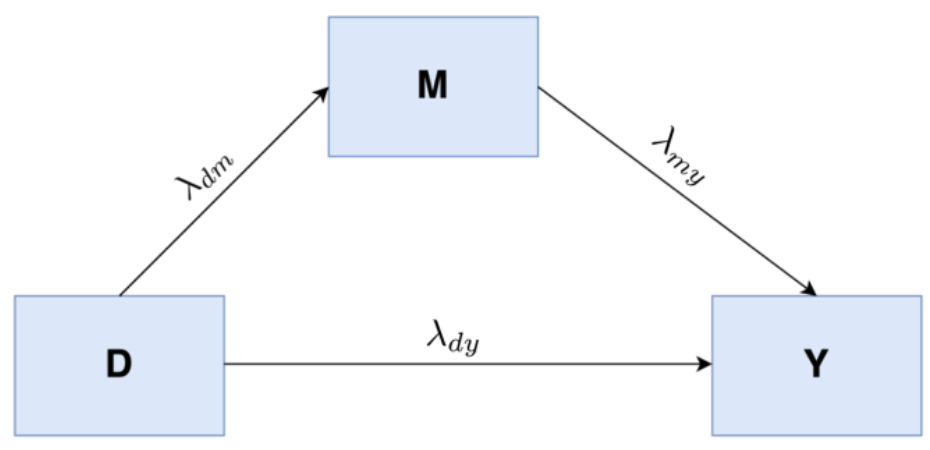
\includegraphics[width=0.6\textwidth]{../input/med_func_form_fig.png}
    \caption{Mediation Graph with Linear Functional Form}
    \label{fig:med_func_form_fig}
\end{figure}

We can then see from either 
the model or the graph that the average indirect 
effect is given by $\lambda_{d m} \lambda_{my}$.
That is, we're scaling the effect of $M$ on $Y$
by how much $D$ affects $M$.

This result has inspired 
many papers to engage in 2-stage experiments 
in which they first randomize $D$ and estimate 
the effects on $M$ and then, in a second 
experiment, randomize
$D$ and measure its effect on $Y$ controlling for 
$M$.

See the appendix of John's book for a demonstration of this.

%%%%%%%%%%%%%%%%%%%%%%%%%%%%%%%%%%%%%%%%%%%%%%%%%%%%%%%%%%%%%%%%%%%%%%%%%%%%%%%%%%%%%%%
%%%%%%%%%%%%%%%%%%%%%%%%%%%%%%%%%%%%%%%%%%%%%%%%%%%%%%%%%%%%%%%%%%%%%%%%%%%%%%%%%%%%%%%
\subsection{Basic Case: Binary Randomized Treatment}

There are alternative approaches available 
when the experimenter is able to directly manipulate $M$.

Given that
$D$ has been randomly assigned, 
we can be confident in the assumption:

\begin{notes}[Assumption: Statistical Independence of the Treatment]
    \begin{align}
        \left\{Y_i(1,1), Y_i(1,0), Y_i(0,1), Y_i(0,0), M_i(1), M_i(0)\right\} \perp D_i
    \end{align}
\end{notes}

We can then consider another assumption:

\begin{notes}[Assumption: Conditional Independence of the Mediator]
    \begin{align}
        \left\{Y_i(1,1), Y_i(1,0), Y_i(0,1), Y_i(0,0)\right\} \perp M_i \mid D_i
    \end{align}

    ``Concretely, this assumption requires that the value of 
    the mediator is as good as randomly assigned, 
    even though the researcher did not have direct 
    control over its level.''
\end{notes}

Putting these together:

\begin{notes}[Assumptions Combined: Sequential Randomization or Sequential Ignorability]
    Researchers typically consider the above two assumptions jointly 
    as the assumption of sequential randomization or sequential ignorability:

    \begin{align}
        &\left\{Y_i(1,1), Y_i(1,0), Y_i(0,1), Y_i(0,0)\right\} \perp M_i \mid D_i \\
        &\left\{Y_i(1,1), Y_i(1,0), Y_i(0,1), Y_i(0,0), M_i(1), M_i(0)\right\} \perp D_i
    \end{align}
\end{notes}

\begin{notes}[Assumption: Support]
    An additional assumption is 

    \begin{align}
        1>\mathbb{P}\left[D_i=1 \mid M_i=m\right]>0 \text { for all } m
    \end{align}

    That is, for all values of the mediator, 
    there is a positive probability of receiving the treatment.
\end{notes}

Under these 3 assumptions, we can 
identify all of the 4 parameters of interest.

For example, under these assumptions, $\mathbb{E}\left[Y_i\left(M_i(1), 0\right)\right]$,
the average outcome if the mediator were the value under treatment
but treatment was set to 0, is given by:

\begin{align}
    \mathbb{E}\left[Y_i\left(M_i(1), 0\right)\right]=\mathbb{E}\left[Y_i \cdot\left(1-D_i\right) \cdot \frac{1}{\mathbb{P}\left[D_i=1\right]}\left(\frac{1}{1-\mathbb{P}\left[D_i=1 \mid M_i=m\right]}-1\right)\right]
\end{align}

%%%%%%%%%%%%%%%%%%%%%%%%%%%%%%%%%%%%%%%%%%%%%%%%%%%%%%%%%%%%%%%%%%%%%%%%%%%%%%%%%%%%%%%
\subsubsection{The Assumption that Fails}

However, in practice, the assumption that is likely to fail
is the assumption of conditional independence of the mediator.
Realistically, the mediator value probably reflects 
choice and optimization by the individual, so it's unlikely
that the mediator is as good as randomly assigned given treatment.
E.g., in the Saudi Arabian norms experiment,
this would fail in a world where whether husbands communicate with their 
wives about the norms is at least partially informed by
how likely the information would be to influence their wives' behavior.

\begin{questions}
    Verify that what I wrote in this example is correct.
\end{questions}


%%%%%%%%%%%%%%%%%%%%%%%%%%%%%%%%%%%%%%%%%%%%%%%%%%%%%%%%%%%%%%%%%%%%%%%%%%%%%%%%%%%%%%%
%%%%%%%%%%%%%%%%%%%%%%%%%%%%%%%%%%%%%%%%%%%%%%%%%%%%%%%%%%%%%%%%%%%%%%%%%%%%%%%%%%%%%%%
\subsection{Separate Randomization of Treatment and Mediator}

Another common approach is to conduct 2 experiments where in the first, the 
experimenter
randomizes $D$ and estimates the effect on $M$, and in the second, 
the experimenter randomizes $M$ and estimates the effect on $Y$.

While this method offers some intuitive appeal, it fails to recover 
parameters of interest, such as the AIE.
See \autoref{fig:med_two_exp_failure} below,
which is included in John's book and is a 
reproduction of a table from Imai et al. (2011).

In this example, we 
see that one gets a positive effect of $D$ on $M$ and a positive effect of $M$ on $Y$:
$0.2$ for each. However, the causal mediation effect 
is actually negative: $-0.2$. Why is this? 
The issue lies in which members of the population 
are affected in each case. The positive effect of 
$D$ on $M$ is driven by the sub-population in the first row, those 
with $M_i(0) = 0$ and $M_i(1) = 1$. However, this is the exact 
population for whom the mediator has a negative effect on $Y$, i.e., for whom 
$Y_i(t,0) = 1$ and
$Y_i(t,1) = 0$. Thus, the issue comes from not appreciating 
that the impact of $D$ on $M$ is not applied uniformly across 
the population, and it may be applied to a sub-population 
for whom the effect of $M$ on $Y$ doesn't match the average effect 
across the population. Such an issue would be ruled out by 
the Sequential Ignorability assumption had it applied here.


\begin{figure}[!htb]
    \centering
        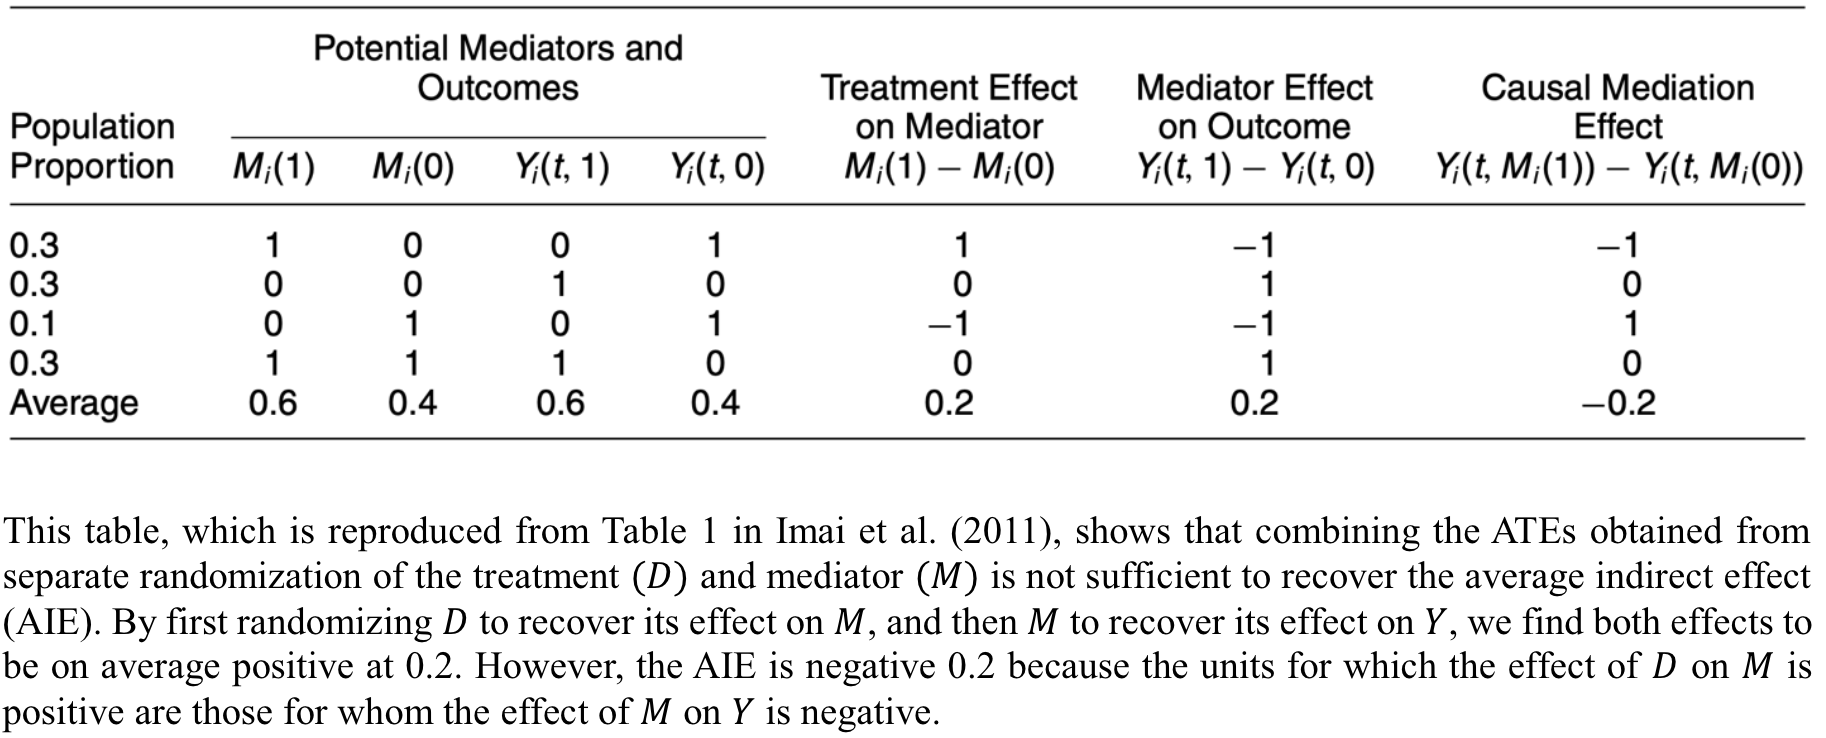
\includegraphics[width=0.9\textwidth]{../input/med_two_exp_failure.png}
    \caption{Separate Randomization of Treatment and Mediator Failing to Recover AIE}
    \label{fig:med_two_exp_failure}
\end{figure}

%%%%%%%%%%%%%%%%%%%%%%%%%%%%%%%%%%%%%%%%%%%%%%%%%%%%%%%%%%%%%%%%%%%%%%%%%%%%%%%%%%%%%%%
%%%%%%%%%%%%%%%%%%%%%%%%%%%%%%%%%%%%%%%%%%%%%%%%%%%%%%%%%%%%%%%%%%%%%%%%%%%%%%%%%%%%%%%
\subsection{Paired Design}




\end{document}